\documentclass[12pt]{article}
\usepackage{amssymb}
\usepackage{amsmath}
\usepackage{graphicx}
\usepackage{amsfonts}
\title{LCS Independent Study Report}
\author{Zheng Liu}
\begin{document}
\maketitle

\section{Abstract}
After a brief study of the background of fluid and LCS, the main work done is simulations of the double gyre model. Based on a skeleton code from previous year, the program was developed to generate and take in data in a friendly csv or txt format. Then, a lot of comparisons between the theoretical results and data generated results were made by experimenting with the simulation. The main results obtained include the conservation of divergence field, error study of velocity field, study of interpolation methods, improvement of computation time, and finally FTLE animation.  

\section{Introduction}
This section briefly introduce motivation and techniques used for each part. First, data generation and input can make the code serve not only as simulation in theory but also a tool for experimental data processing. The formats of the data were chosen so that they are close to the output of typical scientific instruments. It is also easy to tweak the code to accommodate other formats. Second, the velocity field for both theoretical and data generated simulations were plotted. Because to do it, the data needs to be interpolated, the plot is a basic validation. Then a ball was put into both velocity field. Great divergence of their trajectories was seen after some time. This basically shows the integration of the velocity causes small error introduced by interpolation blowing up fast. We can also sort of see the conservation of divergence in this part. Third, the divergence field was calculated because divergence is important for FTLE. Last but not the least, FTLE animation was made for the data generated model. The processing time was improved by processing data in place on memory. The comparison between it and the theoretical model validated how well it worked.    

\section{General Comments on the Code}
To run the code, please make sure Python 3, Numpy, and Matplotlib are installed. Before running, please run pre.sh to prepare the environment. 

Because there are multiple functions, each function is made a separate file. Please make sure the grid and time length (T) of the simulation are consistent through all files.

\section{Results}
\subsection{Data Generation and Input}
\begin{center}
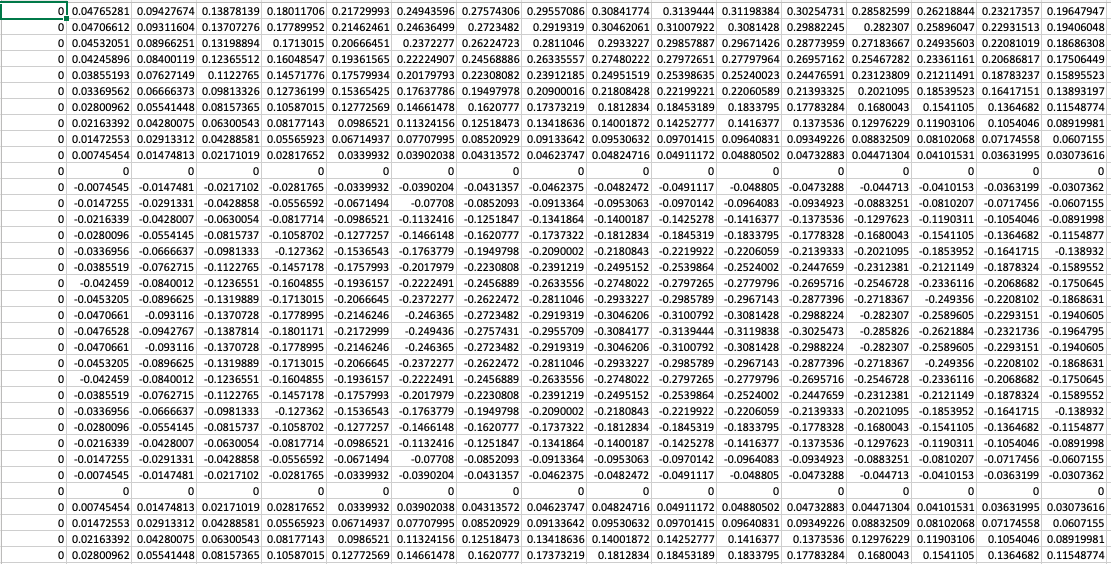
\includegraphics[width=\textwidth]{csvData}
\small Figure 1: Sample generated csv data
\end{center}

\begin{center}
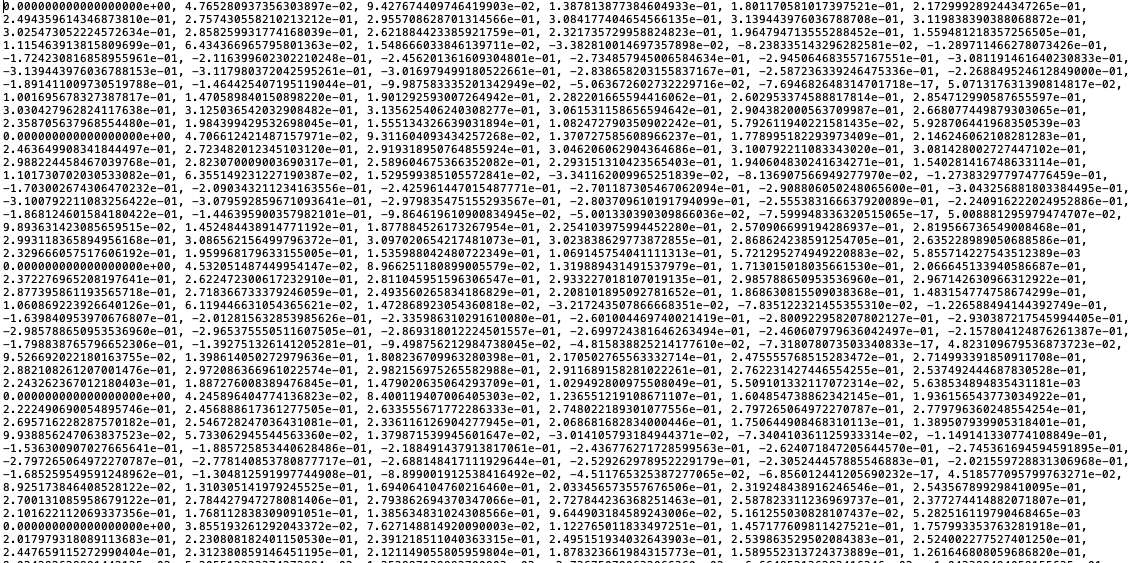
\includegraphics[width=\textwidth]{txtData}
\small Figure 2: Sample generated txt data
\end{center}

Figure 1 shows the generated csv data and Figure 2 shows the sample generated txt data. To generate data, in terminal, run:

\begin{center}
python data.py 
\end{center} 

 

The mode can be selected by user input following the prompt.

The parameters of function $data_gen(x_min,x_max,y_min,y_max,T,op)$ decide the grid and time period of the simulation. Please see comments for details.


\subsection{Velocity Field}
To run this part, use command:

\begin{center}
python interp\_vField.py 
\end{center} 

\begin{center}
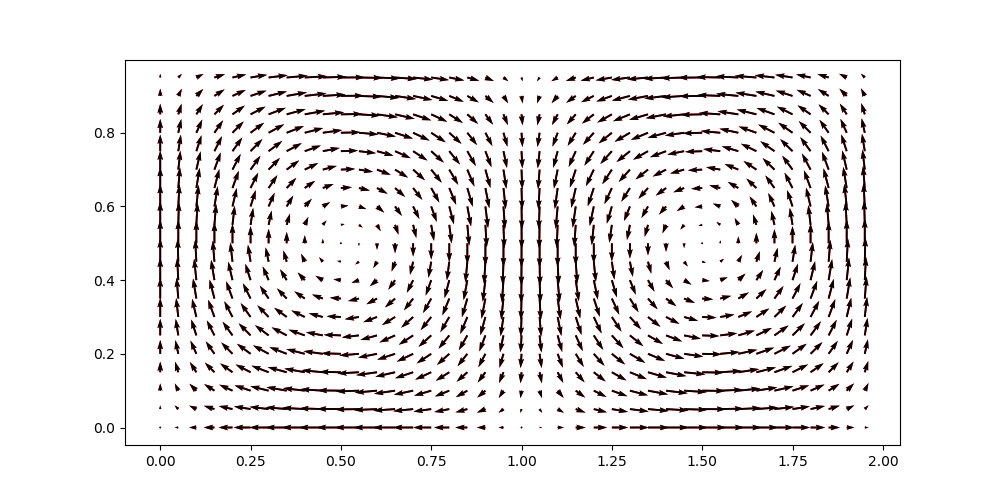
\includegraphics[width=\textwidth]{field}
\small Figure 3: Plotted velocity field by data and model (overlapped).
\end{center}

Figure 3 shows the field generated by model and the data on top of each other. The red arrows are for data and black arrows are for model. We can see that they are almost identical because they perfectly overlap. This proves that interpolation works fine.



\subsection{Motion of a Point in Field}
To run this part, use command:

\begin{center}
python double\_gyre.py 
\end{center} 

And then type in the coordinates for two balls. Please note that there are positions that make balls only move horizontally or vertically due to the field.

A ball (point) is put into the velocity field formed by the double gyre model. On top of that, another layer of the same plot is drawn but with everything from data. The color coding stays consistent. The green arrow represents the distance of two balls (it is a vector).

\begin{center}
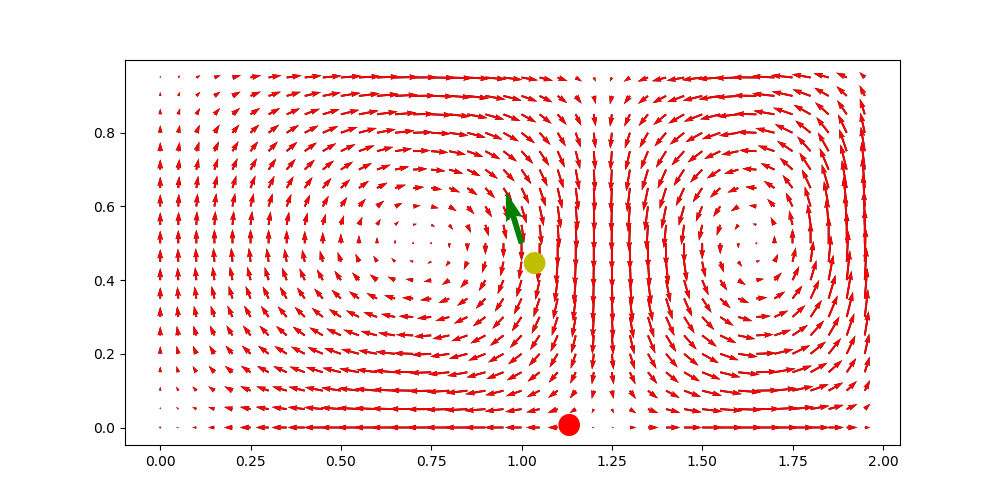
\includegraphics[width=\textwidth]{ball}
\small Figure 4: Snapshot of moving ball gif
\end{center}


From the gif included (snapshot in Figure 4), we can see that the two balls separate soon after initialization. The cause of that was studied by using higher precision number objects in python and trying other interpolation schemes. But later I found out that the trajectories diverge even for balls both from the same generated data. Therefore, it is a chaotic behavior. It was confirmed that Jialun Bao observed the same results. This might be more interesting for some other dynamic systems that don't cause chaotic behaviors.


\subsection{Divergence Calculation}
To run this part, use command:

\begin{center}
python div.py
\end{center} 
Then pick the time you want to see the divergence at. The printed result is output into div.txt.

The divergence fields of two cases (model and data) are both printed and plotted. It is clear that the divergence of two cases is almost zero everywhere. The plot in Figure 5 shows the distribution of tiny divergence values in the field. The values for two cases are very close.

Please note that although at t=0, the divergence can  be e-14, later it does get larger to e-4. Animation was not made due to time, but a test was conducted to make sure divergence is always small everywhere. 

\begin{center}
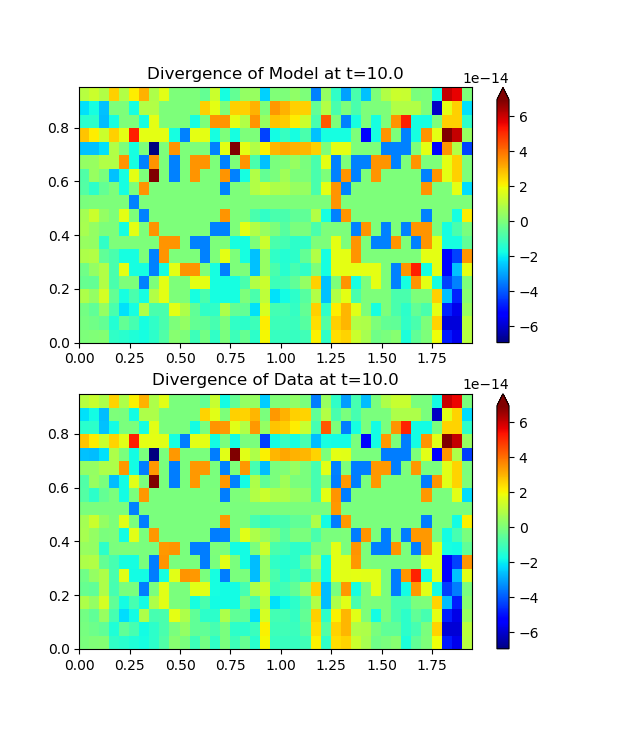
\includegraphics[width=\textwidth]{div}
\small Figure 5: Divergence field plot
\end{center}

\subsection{FTLE Animation}
To run this part, use command:

\begin{center}
python mapping.py\\
python FTLE.py \\
python animation.py\\
\end{center} 
The first two generate necessary files for the animation and take a while. Only run animation.py if no need to update model or data.

The animation shows the FTLE field for each case. In the included gif file (snapshot in Figure 6), they look the same when generating perfect data. The interpolation did not introduce much error at this stage. So there is a potential for interpolating data to raise resolution. Overall the interpolation does not scramble the results. Further work may be adding noise in data generation to see how everything reacts.

\begin{center}
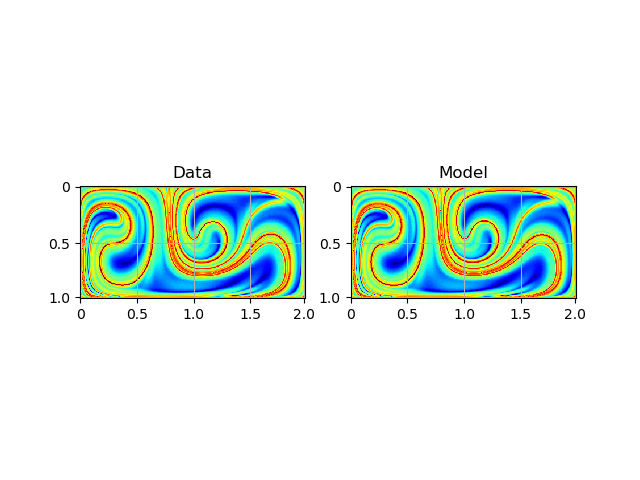
\includegraphics[width=\textwidth]{FTLE}
\small Figure 6: Snapshot of FTLE field gif
\end{center}

   

\end{document}